\documentclass[a4paper,UTF8]{article}
\usepackage[UTF8]{ctex}
%\usepackage{ctex}
\usepackage[margin=1.25in]{geometry}
\usepackage{color}
\usepackage{graphicx}
\usepackage{amssymb}
\usepackage{amsmath}
\usepackage{amsthm}
%\usepackage[thmmarks, amsmath, thref]{ntheorem}
\theoremstyle{definition}
\newtheorem*{solution}{Solution}
\newtheorem*{prove}{Proof}
\usepackage{multirow}
\usepackage{url}
\usepackage[colorlinks,urlcolor=blue]{hyperref}
\usepackage{enumerate}
\renewcommand\refname{参考文献}


%--
\begin{document}
\title{\textbf{《计算机图形学》四月报告}}
\author{161240056,谈婧,\href{mailto:jingtan@smail.nju.edu.cn}{jingtan@smail.nju.edu.cn}}
\maketitle

\section{综述}
本系统为一个包含了图形学用户界面程序和命令行界面程序的绘图系统。本绘图系统包含如下功能函数:重置画布、保存画布、设置画笔颜色、绘制线段绘制多边形、绘制椭圆、绘制曲线、对图元平移、对图元旋转、对图元缩放、对线段裁剪。

\section{算法介绍}
\subsection{重置画布ResetCanvas}
重置画布函数的声明为resetCanvas(width, height, canvas)。
本函数为了实现对于参数中注明的画布Canvas的重定义大小,采用了canvas控件的bind方法,与"<Configue>"绑定,以此进行Canvas的长宽重定义。首先改变canvas的width和height属性大小,再使用canvas的config函数重定义canvas大小。
\subsection{\dots}
\dots
		
\section{系统介绍}
本系统使用python3.6开发,图形学用户界面程序由python tkinter package支持开发。本系统中的绘图核心算法在`/algorithms.py`中实现。对于每个绘图算法,除了必要的绘图所需参数传递外,增添了画布参数,方便确认需要图形绘制的特定画布。由于图形学用户界面不会和命令行界面发生交互,因此在本系统中图形学用户界面和命令行界面的实现过程中会各自自行定义画布。
\subsection{图形学用户界面设计说明}
本用户界面包含了一个App类,类在初始化时会调用每个绘图函数方法,实现各种函数调用组件,获取参数并调用algorithms.py中的核心算法绘图。
界面预览如下图:

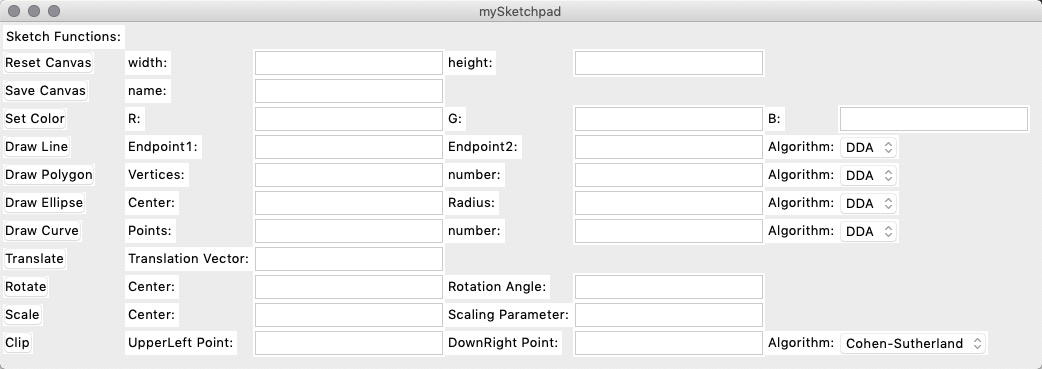
\includegraphics[width=12cm, height=5cm]{picture/gui_1st.jpg}

本界面主要包含两个Tk窗口,分别为root和board。root中包含函数调用按钮,board则为绘图展示窗口。root的设计结构中包含一个Frame组件(mainframe),用于承载各种零碎部件。在mainframe中主要包含Button、Entry、Label和OptionMenu组件,其中Button组件用于完成算法执行按钮的设置,位置分布在最左边一栏;Entry组件用于完成需要键入文本的部分;Label组件和Entry组件搭配使用,用于提示需要键入的文本类型和内容;OptionMenu组件用于设计绘图所需Algorithm的下拉菜单。Board中主要包含一个Canvas控件,用于展现绘图结果\cite{1}。

\section{总结}
\dots

@MISC{WEBSITE:1,
	HOWPUBLISHED = "\url{http://effbot.org/tkinterbook/}",
	AUTHOR = "Intel",
	TITLE = "An Introduction to Tkinter",
	MONTH = "Nov",
	YEAR = "2005",
	NOTE = "Accessed on 2019-04-13"
}
\section{参考文献}
\bibliographystyle{plain}
	\bibliography{An Introduction to Tkinter}
	%http://effbot.org/tkinterbook/
	\bibliography{tkdocs}
	%, https://tkdocs.com/tutorial/
	\bibliography{技术博客:python – 如何让tkinter画布动态调整窗口宽度?}
	%, http://www.voidcn.com/article/p-dshhrxln-btr.html
	\bibliography{python Tkinter Programming tutorial}
	%, https://www.tutorialspoint.com/python3/python_gui_programming.htm


\end{document}